\documentclass{article}
\usepackage{graphicx} % Required for inserting images
\usepackage{subcaption}
\usepackage[backend=biber, sorting=none]{biblatex}
\title{Case Report}
\author{adriencanterot}
\date{June 2023}
\addbibresource{references.bib}
\begin{document}
\maketitle

\section{Background}
Immune checkpoint inhibitor (ICI) in non small cell lung cancer (NSCLC) has been shown to improve overall survival and is the standard of care in the first line setting whether the disease is locally advanced or metastatic.
However, immune related adverse events (irAE)  are frequent and can be severe. Most common irAE are dermatological, gastrointestinal, endocrine, hepatic, and pulmonary. The incidence of pulmonary IrAE is 3.1\% \cite{ramos-casals_immune-related_2020}

Pulmonary Langerhans cell (LC) histiocytosis (PLCH) has unknown cause and is a rare neoplastic disorder characterized by the infiltration of lungs and various organs by bone marrow-derived Langerhans cells with an accompanying strong inflammatory response. These cells carry somatic mutations of BRAF gene and/or NRAS, KRAS, and MAP2K1 genes, which cause activation of the mitogen-activated protein kinase (MAPK)/extracellular signal-regulated kinase (ERK) signaling pathway. PLCH occurs predominantly in young smokers, without gender predominance. \cite{radzikowska_update_2021}
Symptoms are variable, ranging from asymptomatic to cough, dyspnea, chest pain, and hemoptysis.
Radiologically, it can present as nodules, cysts, or a combination of both. 

The clinical presentation is variable, ranging from a single bone lesion to multisystem disease. The diagnosis is based on the presence of Birbeck granules on electron microscopy, CD1a and CD207 (Langerin) expression on immunohistochemistry, and the presence of BRAF V600E mutation. The treatment depends on the extent of the disease and the organ involved. The prognosis is variable, ranging from spontaneous resolution to death. Tobacco plays an important role in the resolution of symptoms.

We report a case of Langerhans cell histiocytosis (LCH) after treatment with durvalumab for non small cell lung cancer (NSCLC).

\section{Case presentation}
We report the case of a 58 year old patient with priors of stroke, patent foramen ovale. Current smoker.
Diagnosed with locally advanced adenocarcinoma (PDL1 score 0\%, insufficient material for molecular biology) staged as cT2aN3M0 with a tumor size of 37mm, ipsilateral mediastinal lymph nodes and contralateral mediastinal lymph nodes. (4L and 4R, 7) according to ACJCC 8th edition \cite{goldstraw_iaslc_2016}.

The patient was treated with radiochemotherapy (66Gy in 33 fractions with carboplatin AUC 5 and paclitaxel 90mg\/m2 weekly for 6 cycles) followed by 13 cycles of durvalumab (10mg\/kg every 2 weeks). Following CT scan showed a partial response according to RECIST 1.1 criteria.

Starting cycle 11 of treatment, the patient developed a grade 2 cough, grade 2 dyspnea and grade 2 fatigue. Following CT scan showed the emergence of diffuse micronodulation predominantly observed in the upper lobes. \ref{fig:scan2}
The patient was initially treated with prednisone 1mg\/kg\/day for 1 month with no improvement to the symptoms following the GERMOP protocol. \cite{lazor_cryptogenic_2000}
The CT scan at 3 month follow-up showed a worsening of the micronodulation and the emergence of cysts. (Figure \ref{fig:scan3})

\begin{figure}[ht]
  \centering
  \begin{subfigure}[t]{0.45\linewidth}
    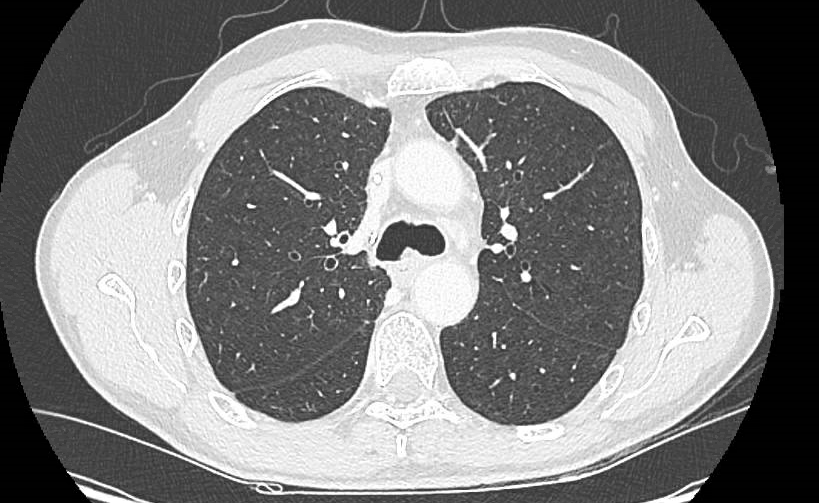
\includegraphics[width=\linewidth]{scan-before.png}
    \caption{Before treatment}
    \label{fig:scan1}
  \end{subfigure}
  \begin{subfigure}[t]{0.45\linewidth}
    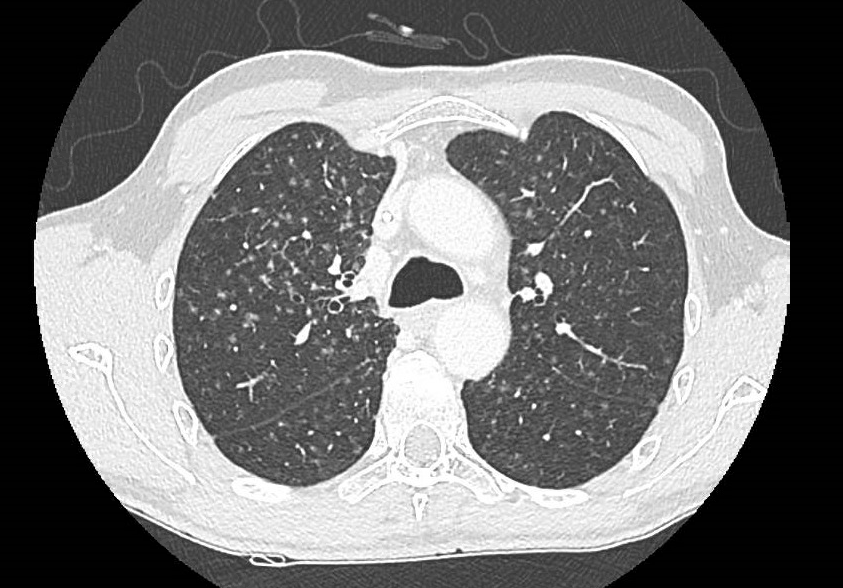
\includegraphics[width=\linewidth]{scan-m0.png}
    \caption{First appearance at cycle 11}
    \label{fig:scan2}
  \end{subfigure}
  \begin{subfigure}[t]{0.45\linewidth}
    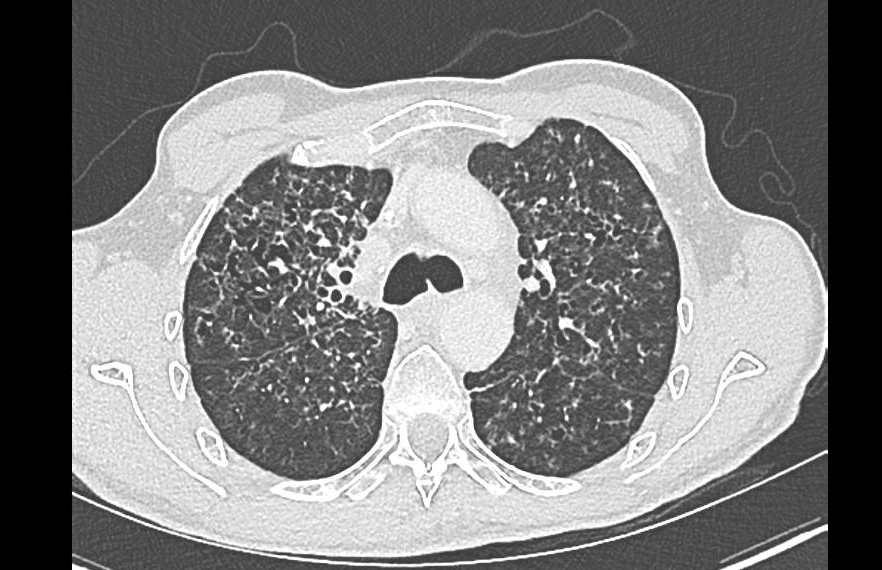
\includegraphics[width=\linewidth]{scan-m3.png}
    \caption{Worsening at 3 month follow up}
    \label{fig:scan3}
  \end{subfigure}
  \begin{subfigure}[t]{0.45\linewidth}
    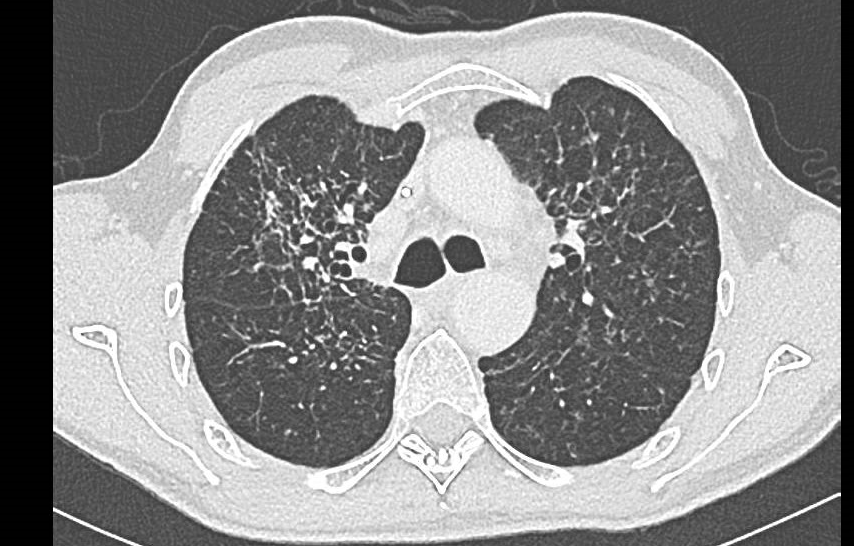
\includegraphics[width=\linewidth]{scan-m6.png}
    \caption{Improvement at 6 month follow up}
    \label{fig:scan4}
  \end{subfigure}
  \caption{CT scans}
\end{figure}
  


A bronchoscopy was then performed and showed a normal bronchial tree. The bronchoalveolar lavage was polymorphous with 14\% of lymphocytes. The transbronchial biopsy showed a normal lung parenchyma with no sign of inflammation or fibrosis. The transbronchial biopsy was negative for CD1a and CD207 (Langerin) expression on immunohistochemistry. The transbronchial biopsy was negative for BRAF V600E mutation. 
Lung function was preserved with no sign of obstructive or restrictive syndrome. TLCO was 40\% of predicted value. He did not present hypoxemia at rest.

Maintenance immunotherapy was stopped after 13 cycles due to the worsening of the symptoms and the CT scan. 

At 6 month follow up, clinical evaluation showed a major reduction in symptoms with no cough and no dyspnea. It is important to note that the patient stopped smoking 10 days before the CT scan and switched for a nicotin based electronic cigarette.
The CT scan showed a major reduction in micronodulation and cysts. (Figure \ref{fig:scan4})

The patient maintained the benefits after 6 months of follow up and the CT scan showed an almost complete resolution of the micronodulation and cysts.

\section{Discussion}
\subsection{Langerhans cell histiocytosis diagnosis}
The diagnosis was made on the clinical presentation and the radiological findings. The bronchoscopy and the transbronchial biopsy were negative for CD1a and CD207 (Langerin) expression on immunohistochemistry. The transbronchial biopsy was negative for BRAF V600E mutation.
It was a probable diagnosis of pulmonary Langerhans cell histiocytosis. A definite diagnosis would have required a CT guided biopsy or a surgical biopsy. However, the patient was asymptomatic and the CT scan showed a major improvement. 

However, the rapidly appearance of the micronodulation and cysts after the start of durvalumab and the rapid improvement after the stop of durvalumab strongly suggest that the pulmonary Langerhans cell histiocytosis was related to durvalumab.

Even though the biopsies did not show any sign of Langerhans cell histiocytosis, they did not show any differential diagnosis such as sarcoidosis, hypersensitivity pneumonitis, or other interstitial lung diseases either. Bronchoalveolar lavage was not in favor of an active infection.

\subsection{Langerhans cell histiocytosis and immune checkpoint inhibitors}
To our knowledge, there is no case of Langerhans cell histiocytosis after treatment with immune checkpoint inhibitors. 
However, there are number of cases of hemophagocytic lymphohistiocytosis (HLH) after treatment with ICI. \cite{sadaat_hemophagocytic_2018, takeshita_coincidence_2017, noseda_haemophagocytic_2019}

Recent studies on pulmonary Langerhans cell histiocytosis have shown that neoplastic histiocytosis cells can over express PD-L1.
Galatica et al. showed overexpression of PD-L1 in extrapulmonary forms of Langerhans cell histiocytosis.

Wang et. al. showed elevated PD-1 expression (100\%) and low PD-L1 expression (33\%) in pulmonary Langerhans cell histiocytosis in a cohort of 6 patients.

Langerhans cell microenvironment might play a role in immunotherapy toxicity. Further studies are needed to better understand the role of Langerhans cell microenvironment in immunotherapy toxicity.

\section{Conclusion}
We report a case of probable pulmonary langerhans cell histiocytosis after treatment with durvalumab for non small cell lung cancer. The diagnosis was made on the clinical presentation and the radiological findings. The bronchoscopy and the transbronchial biopsy were negative for CD1a and CD207 (Langerin) expression on immunohistochemistry. It was a probable diagnosis of pulmonary Langerhans cell histiocytosis.
Langerhans cell microenvironment might play a role in immunotherapy toxicity. Further studies are needed to better understand the role of Langerhans cell microenvironment in immunotherapy toxicity.

\printbibliography
\end{document}


\section{Abreviations}
\begin{itemize}
\item ICI: immune checkpoint inhibitors
\item NSCLC: non small cell lung cancer
\item irAE: immune related adverse events
\item PD-L1: programmed death ligand 1
\item PD-1: programmed death 1
\item CTLA-4: cytotoxic T-lymphocyte-associated protein 4
\item HLH: hemophagocytic lymphohistiocytosis
\item CT: computed tomography
\item TLCO: transfer factor of the lung for carbon monoxide
\item ACJCC: American Joint Committee on cancer
\item RECIST: Response Evaluation Criteria in Solid Tumors
\end{itemize}
